\section{SwissCat+}
Les catalyseurs sont une espèce chimique qui permet ou accélère la réaction chimique sans être consumé dans le processus. Les catalyseurs sont utilisés dans divers domaines (Agricole, militaire, chimie, traitements des déchets, transformation de polluants, \dots). Ils sont indispensables dans notre société cependant, ces produits requièrent souvent des terres rares. Par exemple, les catalyseurs dans les voitures (qui servent à réduire les émissions de gaz polluants en transformant notamment le monoxyde de carbone, les hydrocarbures imbrûlés et l'oxyde d'azote en eau, dioxyde de carbone et dioxyde d'azote) sont composés d'alumine, d'oxyde de cérium, mais surtout, ils sont composés d'au moins trois platinoïdes.

C'est dans ce contexte de réduction d'utilisation de terres rares que le laboratoire SwissCat+, a été créé dans le but d'optimiser la composition des catalyseurs et d'en trouver de nouveaux. Le laboratoire est scindé en deux, le laboratoire Est, situé à l'ETHZ à Zurich, s'occupe de faire des recherches sur les catalyseurs hétérogènes, tandis que la partie du laboratoire Ouest, située à l'EPFL à Lausanne, fera des recherches sur les catalyseurs homogènes.
\subsection{Laboratoire ouest}
Pour augmenter la cadence et la précision du système, le laboratoire doit être automatisé. Cela permettra également de faire gagner du temps aux chimistes sur les tâches répétitives et à faible valeur ajoutée.
Le laboratoire doit posséder une partie de \gls{synthese}, qui sert à réaliser les expériences, pour ce faire, il doit pouvoir manipuler des matières liquides et de larges quantités de solides ($\qtyrange[range-units=single]{0.1}{50}{\mg} $). Il possédera également une partie analyse qui servira pour examiner le résultat des expériences réalisées en amont.

\section{Contexte et objectifs du projet Storm}
Dans le cadre de l'automatisation de la chimie synthétique à haut débit, la distribution précise de petites quantités ($\leq \qty{1}{\mg}$) représente un défi technologique majeur. Actuellement, cette tâche repose sur des itérations successives de collecte et de dosages de minuscules quantités, un processus non seulement chronophage lorsqu'il s'agit de mener de vastes séries d'expériences, mais c'est également un processus sujet à des contaminations croisées tout en nécessitant une quantité importante de matière. En raison de la diversité des propriétés des solides, cette méthode peut rapidement devenir complexe, voire impossible. Aucune solution universelle n'existe.
C'est dans ce cadre que le projet STORMS (\textit{STOchasitic Robotized Micro Sampling}). Il est réalisé en collaboration entre l'EPFL, l'HEIG-VD, Chemspeed Technologies et Dietrich Engineering Consultants (DEC).
STORMS est implémenté dans une plateforme de \gls{synthese}. Cette plateforme possède $7$ modules dont $4$ appartiennent à STORMS : 
\begin{itemize}
    \item la standardisation,
    \item le stockage,
    \item le micro-échantillonnage (\textit{microsampling}),
    \item la recombinaison
\end{itemize}
\begin{figure}[h]
    \centering
    \includegraphics{assets/figures/schema_storms.drawio}
    \caption[Schema des modules de la platforme de \gls{synthese}]{Schéma des modules de la plateforme de \gls{synthese}. En bleu les \glspl{glovebox} du projet STORMS, en rouge celles de la \gls{synthese}.}
    \label{fig:schema_module_storms}
\end{figure}
La standardisation a pour but de donner des récipients de taille standard aux microsampling qui va créer des \gls{microcapsule}.
Les \glspl{microcapsule} peuvent contenir de $\qtyrange[range-units=single]{0.1}{10}{\mg}$ de produit. Dû aux grandes différences de caractéristiques des produits à expérimenter, il n'est pas possible de déterminer précisément à l'avance la quantité qui sera délivrée dans les \glspl{microcapsule} par le \textit{microsampling}.
Les \glspl{microcapsule}, une fois fabriquées, sont pesées puis mises sur des plaques nommées \glspl{wellplate}, qui sont ensuite stockée. Le stockage fait lien entre la standardisation, le \textit{microsampling} et la recombinaison.
La recombinaison doit réaliser les \glspl{recette} voulues à partir du stock disponible avant d'envoyer les réacteurs dans les \glspl{glovebox} suivantes pour la \gls{synthese} (\cf \autoref{img:schema_fonct}).
\begin{figure}[H]
    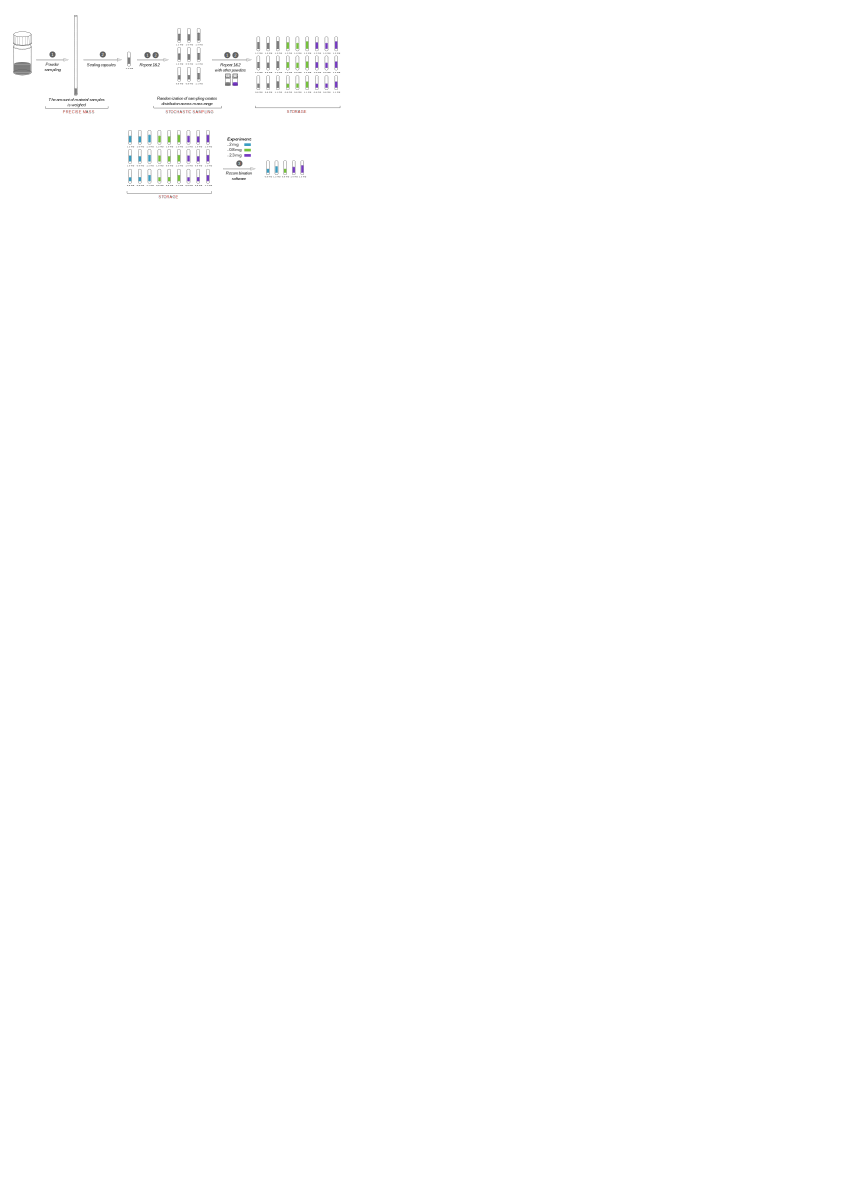
\includegraphics[width=\linewidth]{assets/figures/schema_fonct.svg}
    \caption{Schéma de fonctionnement de STROMS}
    \label{img:schema_fonct}
\end{figure}

\section{Recombinaison de microcapsules}
Le processus de recombinaison consiste à assembler différentes \glspl{microcapsule} de poudres pour répondre aux besoins expérimentaux. Le logiciel de recombinaison sélectionne parmi les \glspl{microcapsule} disponibles afin d'obtenir une composition entrant dans les tolérances de quantités pour une expérience donnée. Le but est de maximiser le nombre d'expériences réalisées. Une fois les \glspl{microcapsule} sélectionnées, la \gls{glovebox} recombinaison doit placer ces \glspl{microcapsule} dans les réacteurs correspondant aux \glspl{recette} réalisées.